\part{Внутренне устройство python}

\section{Структуры под капотом}

\subsection{Внутреннее устройство словарей}
\subsection{Внутреннее устройство множеств}
\subsection{Внутреннее устройство списков}
\subsection{Внутреннее устройство таплов}
\subsection{Внутреннее устройство строк}

\section{Как работает GIL}

\subsection{Освобождение памяти}

\subsubsection{Алгоритм подсчета ссылок}
\subsubsection{Сборщик мусора и его поколения (gc generations) или обработка циклических ссылок}

\section{Размеры объектов Python}

\begin{figure}[h!]
\centering
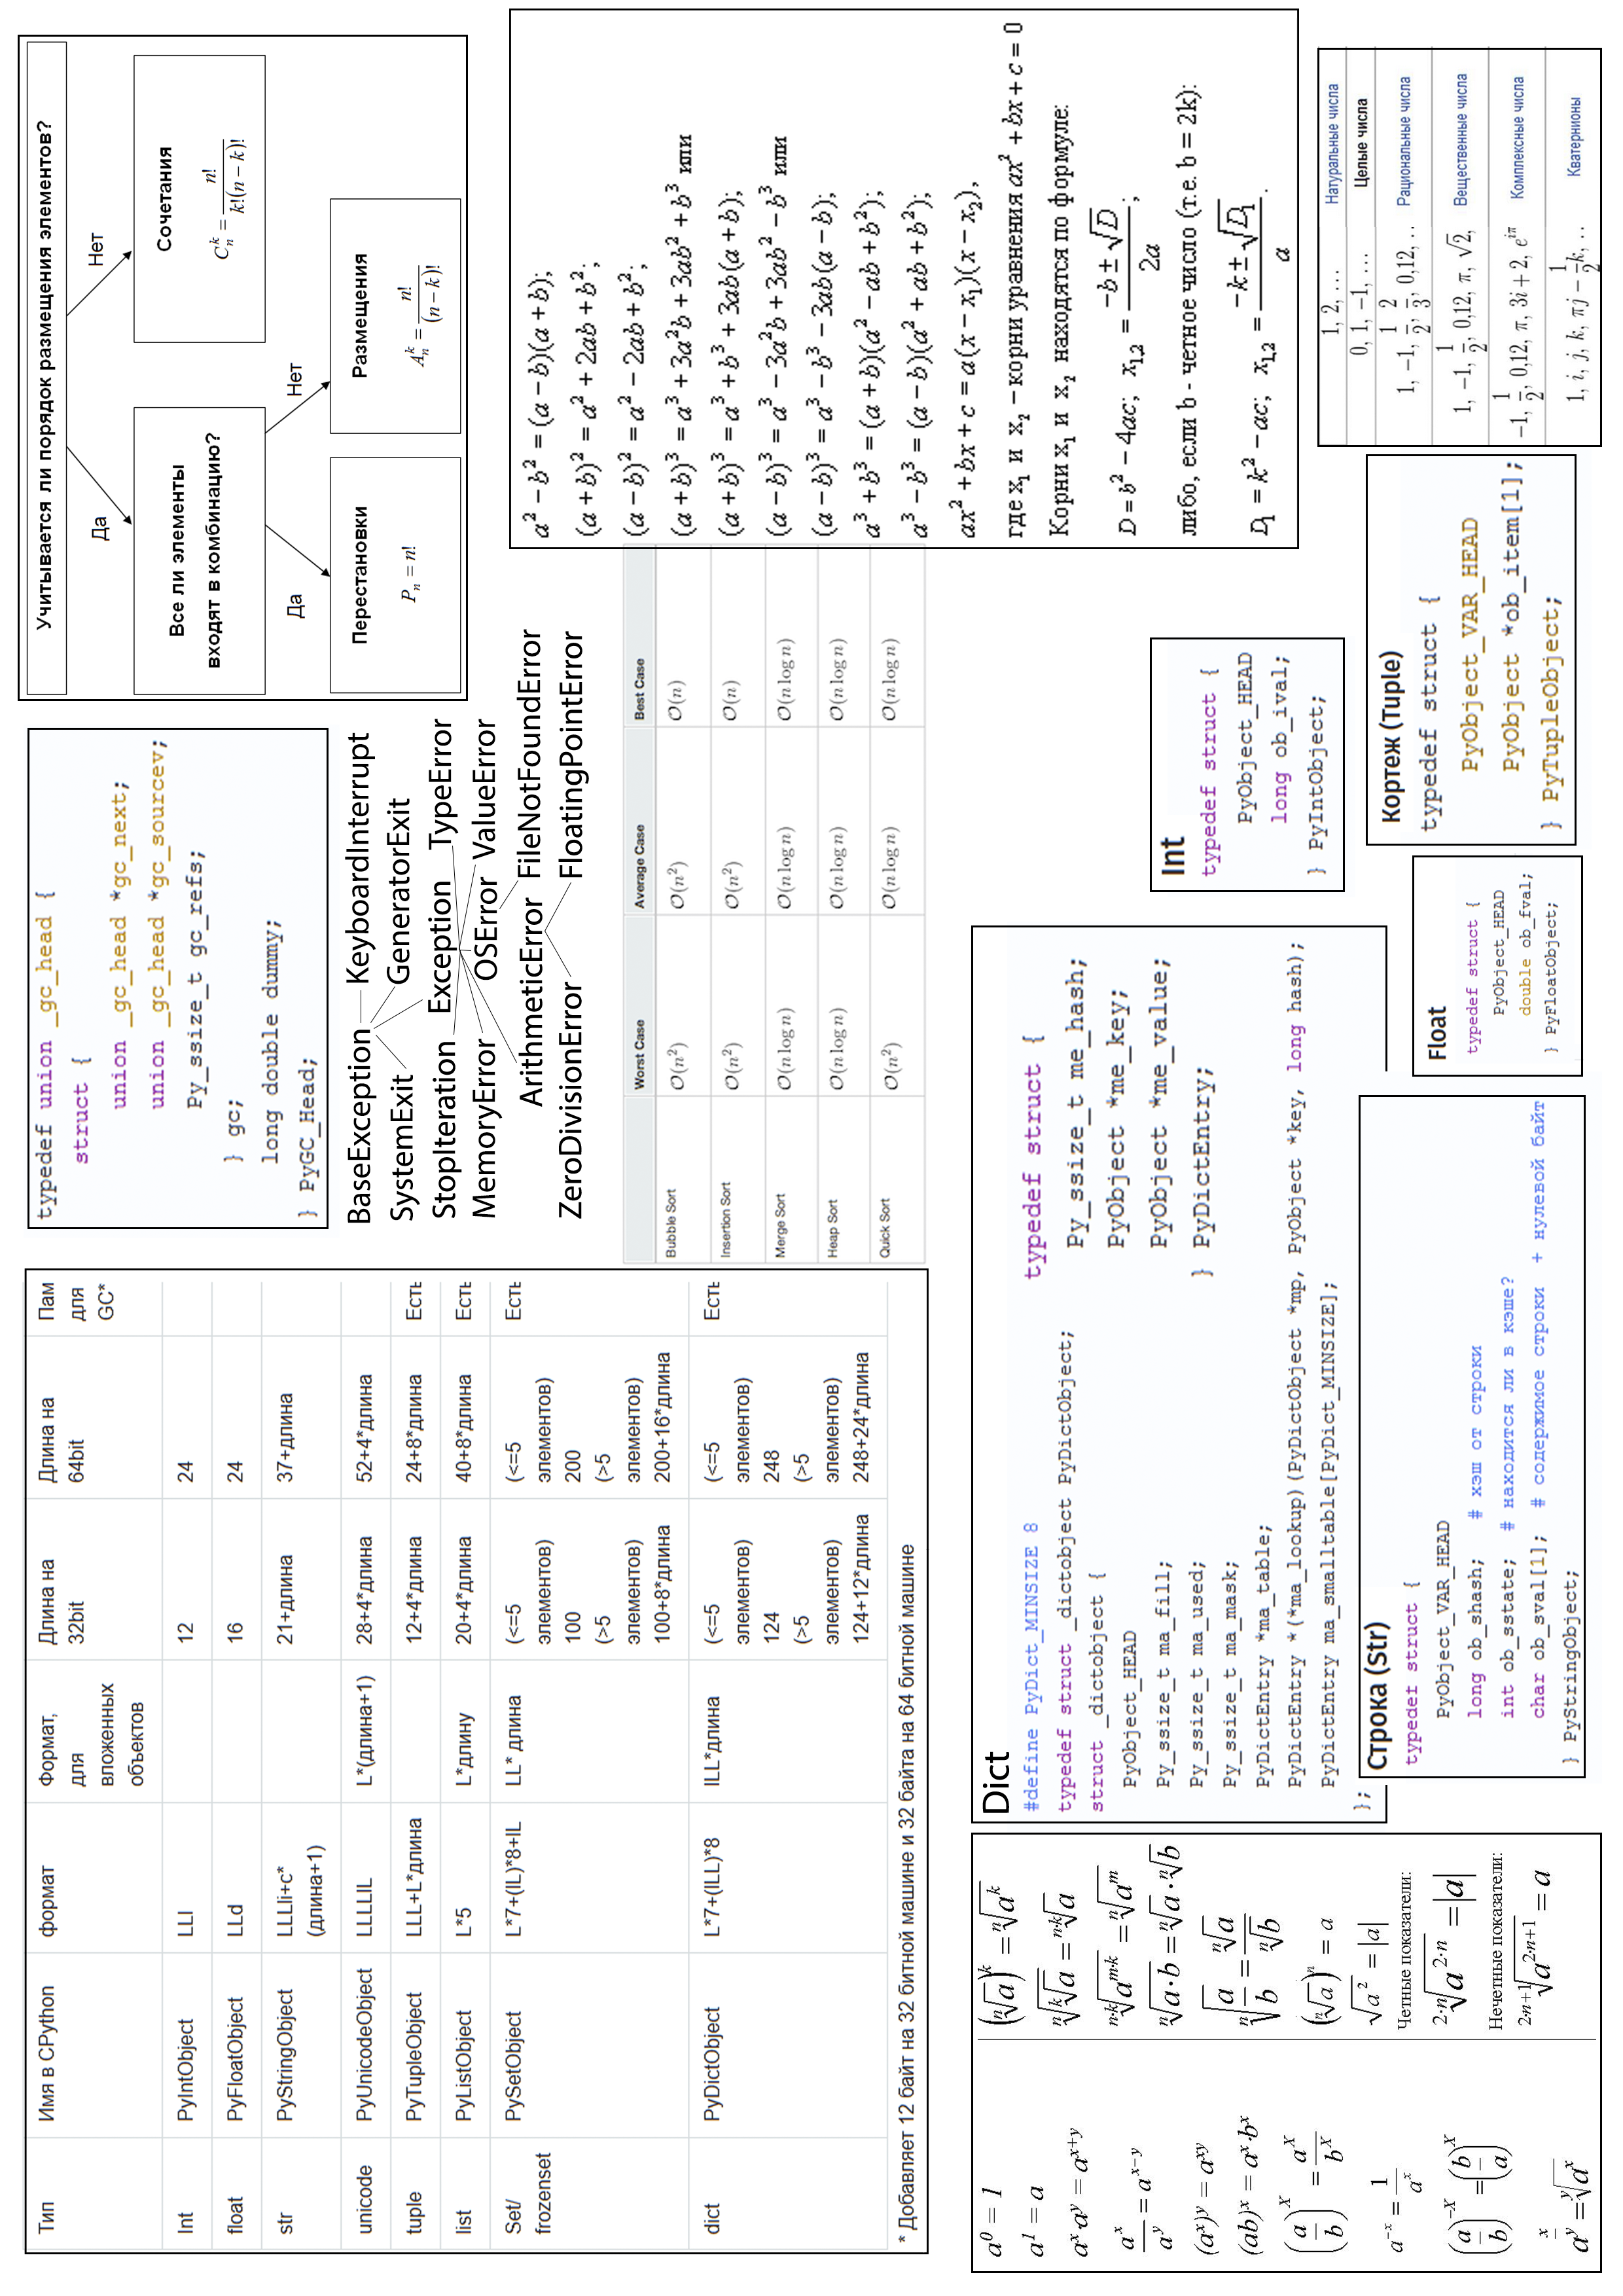
\includegraphics[width=0.8\textwidth]{img/py_data_size.png}
\caption{Размеры объектов в Py}
\label{unicast}
\end{figure}